%%%%%%%%%%%%%%%%%%%%%%%%%%%%%%%%%%%%%%%%%%%%%%%%%%%%%%%%%%%%%%%%%%%%%%%%
\documentclass[a4paper,10pt]{article}
\usepackage[top=1in,bottom=1.25in,left=1in,right=1in]{geometry}
\usepackage{amsmath,amssymb,amsfonts,amsthm}
\usepackage{tabularx}
\usepackage{ae}
\usepackage[T1]{fontenc}
\usepackage{multirow}
\usepackage{graphicx}
\usepackage{sidecap}
\usepackage[dvipsnames]{xcolor}
\usepackage[colorlinks=true,linkcolor=NavyBlue,citecolor=ForestGreen,urlcolor=NavyBlue]{hyperref}

\renewcommand{\rmdefault}{phv}
\renewcommand{\sfdefault}{phv}

%%%%%%%%%%%%%%%%%%%%%%%%%%%%%%%%%%%%%%%%%%%%%%%%%%%%%%%%%%%%%%%%%%%%%%%%
\title{User Manual for gevolution}

\author{Julian Adamek}

\date{\today}
%%%%%%%%%%%%%%%%%%%%%%%%%%%%%%%%%%%%%%%%%%%%%%%%%%%%%%%%%%%%%%%%%%%%%%%%

\hyphenation{Hubble}

\begin{document}

\centerline{\textbf{\huge User Manual for \textit{gevolution} v1.1}}
\vspace{1cm}
\centerline{\large Julian Adamek}
\medskip
\centerline{\today}

\tableofcontents

\section{Preface}

\paragraph{What \textit{gevolution} is and what it isn't.} \textit{gevolution} is a particle-mesh (PM) N-body code which is
specifically designed to provide a general relativistic (GR) treatment of gravity. In order to allow for large simulations, the code uses
massive parallelization based on the MPI protocol. However, very little knowledge about parallel computing is required for the user, as the
entire overhead is hidden inside the \textit{LATfield2} library \cite{David:2015eya}. \textit{LATfield2} provides a framework for managing
data, in particular
\textit{Fields} on a three dimensional regular \textit{Lattice}. The data is automatically distributed over MPI processes using a
rod-decomposition of the three-dimensional domain, i.e.\ two of the three dimensions are scattered over a two-dimensional process grid.
\textit{LATfield2} also has a highly scalable implementation of the three-dimensional Fast Fourier Transform (FFT). In addition, a
versatile \textit{Particle} handler is also provided.

As a consequence of relying on \textit{LATfield2} for all the parallelization and data handling, \textit{gevolution} is a relatively
lightweight code which should be easy to read, understand, and eventually modify. The relativistic formulation and treatment of the laws
of physics allows for the consistent implementation of many theoretical models beyond the baseline $\mathsf{\Lambda}$CDM cosmological
model which comes with this release version of the code. \textit{gevolution} is intended to be a versatile tool for cosmologists who want
to explore the consequences of extensions or alternatives to $\mathsf{\Lambda}$CDM, but it can also be used to address certain questions
within the $\mathsf{\Lambda}$CDM model. However, it is \textit{not} intended as a full replacement of existing ``traditional'' N-body codes
(such as \textit{Gadget} \cite{Springel:2000yr,Springel:2005mi} or \textit{RAMSES} \cite{Teyssier:2001cp}): the applications (i.e.\ the
phenomena which can be studied) have some overlap, but they also cover different terrain.

There are two main points to mention in this respect. Firstly, \textit{gevolution} works at fixed (comoving) spatial resolution which is
owed to its \textit{LATfield2} heritage. Other codes often use either a tree algorithm (e.g.\ \textit{Gadget}) or adaptive mesh
refinement (e.g.\ \textit{RAMSES}) in order to resolve small scale structure inside dense regions. At present, \textit{gevolution} has no
means to achieve this. Adaptive mesh refinement could be implemented in the future, but it is not clear that this is the most relevant
path of development. Secondly, no baryonic physics (hydrodynamics) is implemented in this version of \textit{gevolution}. Again, this
domain is left to traditional N-body codes. We want to provide a simple tool for studies of new phenomena mainly related to relativistic 
physics. Once such phenomena are understood separately one can iteratively increase the level of realism by including additional effects of 
known origin.

\paragraph{Additional information.} This user manual provides essential information about the usage of the code (user interface) and its
internal structure. More information about the \textit{LATfield2} framework can be found in \cite{David:2015eya} or on the
\textit{LATfield2} web site, \url{http://latfield.org}. More information about the theoretical underpinning of \textit{gevolution} can
be found in the main code paper \cite{Adamek:2016zes}. If you use \textit{gevolution} for scientific work, we kindly ask you to cite
\cite{Adamek:2015eda} in your publications.

\paragraph{Copyright} \textcopyright~2015--2016~ Julian Adamek (Universit\'e de Gen\`eve \& Observatoire de Paris)

\paragraph{License.} Permission is hereby granted, free of charge, to any person obtaining a copy
of this software and associated documentation files (the ``Software''), to deal
in the Software without restriction, including without limitation the rights
to use, copy, modify, merge, publish, distribute, sublicense, and/or sell
copies of the Software, and to permit persons to whom the Software is
furnished to do so, subject to the following conditions:
  
The above copyright notice and this permission notice shall be included in
all copies or substantial portions of the Software.
  
\textbf{The Software is provided ``as is'', without warranty of any kind, expressed or
implied, including but not limited to the warranties of merchantability,
fitness for a particular purpose and noninfringement. In no event shall the
authors or copyright holders be liable for any claim, damages or other
liability, whether in an action of contact, tort or otherwise, arising from,
out of or in connection with the Software or the use or other dealings in
the Software.}

\subsection{Development since v1.0}

The most important changes to the code are a greatly improved generator for initial conditions (still called
``\texttt{basic}'') which can now generate initial data based on linear transfer functions for each particle
species. It is even possible to link \textit{CLASS} as a library, so that the required transfer functions
can be computed at runtime. Furthermore, several options to treat the baryonic component have been implemented, including
the possibility to treat it as separate N-body ensemble, however without self-interaction.

This release of the code also contains an additional generator for initial conditions
which can be used to set up the initial phase space of non-cold species according to a procedure proposed in \cite{Ma:1993xs}, see
section 5.4.2 of \cite{Adamek:2016zes} for some details. The linear mode functions for $\mathsf{\Phi}$ and $\mathsf{\Psi}$
required for this procedure are obtained directly from \textit{CLASS}.

The main control sequence has been reorganized and the code sections handling output have been moved into
a separate header file in order to make the code easier to navigate. It is now possible to restart a run from hibernation points.

A linear radiation module based on \textit{CLASS} is now available if \textit{CLASS} is linked as a library. It uses the linear transfer
functions from the Boltzmann code to generate a realization of the perturbed radiation field \cite{Adamek:2017xxx}. This method can also
be used to obtain a linear approximation to the effect of massive neutrinos similar to how it is done in \cite{Brandbyge:2008js}, and
the module allows one to prescribe redshift values at which the treatment for a species switches from linear to N-body. 


\section{Compilation}

\subsection{Requirements}

A copy of the \textit{gevolution} code can be cloned from a public \textit{Git} repository:

\url{https://github.com/gevolution-code/gevolution-1.1.git}

\noindent The code is written in C++ and requires the following additional libraries to be installed.

\begin{itemize}
 \item \textit{LATfield2} version 1.1 (\url{https://github.com/daverio/LATfield2.git})
 \item FFTW version 3
 \item GNU Scientific Library (GSL) and the C-language Basic Linear Algebra Subprograms (CBLAS)
 \item HDF5 (use the parallel version for production runs)
\end{itemize}

\noindent Note also that the code does not support serial execution -- it always requires the MPI protocol to run.

\subsection{Makefile options}

Before calling \texttt{make}, you should set the \textit{include} and \textit{library} paths in the \textit{makefile} to point to your installation of \textit{LATfield2} etc., or you should add those paths to the corresponding environmental variables.

Some features of the code are toggled using compiler options.

\begin{itemize}
 \item[] \hspace{-25pt}\texttt{-DBENCHMARK} ~ With this option set, the code will output some benchmarking information (CPU time spent on various code components).
 \item[] \hspace{-25pt}\texttt{-DPHINONLINEAR} ~ With this option set, the equations will be solved taking into account shortwave corrections. In fact, this option should always be used unless you have a model which sources relativistic corrections at linear order and you know what you are doing.
 \item[] \hspace{-25pt}\texttt{-DCHECK\_B} ~ With this option set, the code will compute a separate copy of the spin-1 component of the
 metric, B$_\mathsf{i}$. This copy is computed using the alternative of the method chosen for the simulation, e.g.\ it will use the
 momentum constraint if that equation is \textit{not} used in the simulation. This can be useful to check consistency but it requires
 additional memory and computations. The option should therefore primarily be used for diagnostic purposes, especially if one is memory limited.
 \item[] \hspace{-25pt}\texttt{-DHAVE\_CLASS} ~ Use this option to link \textit{CLASS} as a library. This allows computing linear transfer functions ``on the fly'' without having to pass them as input files to the IC generator.
 \item[] \hspace{-25pt}\texttt{-DICGEN\_PREVOLUTION} ~ This option enables an additional IC generator called \texttt{prevolution} which can 
 be used to set up -- or ``pre-evolve'' -- the phase space of non-cold species, e.g.\ massive neutrinos. Note that this generator needs to call \textit{CLASS}.
 \item[] \hspace{-25pt}\texttt{-DH5\_HAVE\_PARALLEL} ~ This option enables the parallel output of HDF5 files in the \textit{LATfield2} 
 library. It requires the parallel version of the HDF5 library to be installed on the system. The parallel output mode should always be used if available, especially for production runs.
 \item[] \hspace{-25pt}\texttt{-DEXTERNAL\_IO} ~ This option enables the I/O server of the \textit{LATfield2} library. Use this capability if you have to write large amounts of data (many snapshots) and only if you know what it means.
\end{itemize}

\noindent In addition, the compiler options \texttt{-DFFT3D} and \texttt{-DHDF5}, which switch on the corresponding features of \textit{LATfield2}, are mandatory settings for \textit{gevolution}.

Please note that the \textit{LATfield2} library is developed to a large extent independently of \textit{gevolution}. If you encounter problems related to \textit{LATfield2}, in particular if you discover some bugs in the library, please contact the developers of \textit{LATfield2} directly, \url{developers@latfield.org}.


\section{Running \textit{gevolution}}

A typical command to run a simulation looks like this:

\begin{itemize}
 \item[] \texttt{mpirun -np 16 ./gevolution -n 4 -m 4 -s settings.ini} 
\end{itemize}

\noindent The command-line parameters \texttt{-n} and \texttt{-m} specify the two-dimensional process grid which should be used by the 
\textit{LATfield2} library for the decomposition of the three-dimensional domain. The product of the two numbers gives the total number of 
processes. Note that each number has to be $\geq$ 2, such that the minimum number of MPI processes is 4. Finally, a settings file has to be 
passed with the command-line parameter \texttt{-s}.

If the code is compiled with the \texttt{EXTERNAL\_IO} flag, two additional command-line options, \texttt{-i} and \texttt{-g}, specify the 
number of I/O processes and the mapping of compute processes onto I/O processes (grouping), respectively.

\subsection{Simulation settings}

The settings file is a simple ASCII file which specifies simulation parameters in the format

\begin{itemize}
 \item[] \textit{<parameter name>} \texttt{=} \textit{<value>} [, \textit{<value2>}, \ldots]
\end{itemize}

\noindent The parser ignores empty lines and anything following a \texttt{\#}-symbol. Note that parameter names are case sensitive and that 
white spaces within parameter names are allowed -- the parameter name extends from the first non-whitespace character to the last
non-whitespace character before the equal sign. In fact, the parser is written as to conform with the syntax of \textit{CLASS}
\cite{Blas:2011rf}, see section \ref{sec:IC} for more details.

\begin{itemize}
 \item[] \hspace{-25pt}\texttt{IC generator = basic} ~ Selects the IC generator to be called at initialization. For efficiency reasons,
 \textit{gevolution} can generate initial data ``on the fly'' which is much faster than reading them from disk. This version of the code
 comes with two different IC generators. The default choice is called \texttt{basic} because it uses linear theory without much
 sophistication. The other generator, called \texttt{prevolution}, is only relevant for setting up the initial phase space of non-cold
 species (if present). A third option is \texttt{read~from~disk}, which will prompt \textit{gevolution} to read an initial snapshot from
 provided files. Other IC generators (e.g.\ written by users) should have their own unique name and should prompt the parser to read
 additional settings if appropriate.
 \item[] \hspace{-25pt}\texttt{template file = sc1\_crystal.dat} ~ Specifies a file (in \textit{Gadget-2} format) containing a homogeneous
 particle template. In the simplest case this can be a regular lattice of particles (a ``crystal''), but one could also use a ``glassy''
 template, for instance. If more than one particle species is present a comma-separated list specifies a separate file for each N-body
 ensemble. The templates are assigned in following order: CDM, baryons (if present as separate N-body ensemble), non-CDM species (e.g.\
 massive neutrinos).
 
 There are four template files already available with this version of the code, corresponding to four different crystal structures.
 \texttt{bcc\_crystal.dat} and \texttt{fcc\_crystal.dat} contain a body-centered cubic and face-centered cubic configuration, respectively,
 with 16 and 32 particles in the template. \texttt{sc0\_crystal.dat} and \texttt{sc1\_crystal.dat} contain a simple cubic template with 64
 particles (4$\times$4$\times$4) each. In the first file, a particle sits at each corner of the template, while in the second file the
 corners are centered between eight particles. This allows one to choose how the particle crystal lattice is aligned with the lattice of the
 simulation.
 \item[] \hspace{-25pt}\texttt{tiling factor = 16} ~ Specifies the number of times the particle template shall be repeated in each direction
 in order to fill the entire simulation volume. Note that this parameter thereby sets the total particle number, as
 \textit{N}$_\mathsf{part}$ = \textit{N}$_\mathsf{template} \times ($\texttt{tiling factor}$)^\mathsf{3}$. If more than one particle species
 is present a comma-separated list specifies a separate number for each N-body ensemble. The assignment is as in \texttt{template file}.
 \item[] \hspace{-25pt}\texttt{PSD samples} ~ Since \textit{gevolution} v1.1 this parameter is \textbf{obsolete}. The size of each N-body
 ensemble is entirely controlled with \texttt{tiling factor}.
 \item[] \hspace{-25pt}\texttt{particle file = ic\_cdm.h5} ~ If initial data is to be read from disk instead of being generated on the fly (i.e.\ if \texttt{IC~generator~=~read~from~disk}) a file containing the initial particle configuration has to be specified. If more than
 one particle species is present a comma-separated list specifies a separate file for each N-body ensemble. The assignment is as in \texttt{template file}.
 
 Note that the particle phase space coordinates should be in Poisson gauge when running a relativistic simulation
 (i.e.\ \texttt{gravity theory = GR})! When you are running a Newtonian simulation (i.e.\ \texttt{gravity theory = Newton}) the
 coordinates should be in N-body gauge instead \cite{Fidler:2015npa}.
 \item[] \hspace{-25pt}\texttt{metric file = ic\_phi.h5} ~ If initial data is to be read from disk instead of being generated on the fly
 (i.e.\ if \texttt{IC~generator~=~read~from~disk}) and when running a relativistic simulation (i.e.\ \texttt{gravity theory = GR}) a file
 containing the initial potential $\mathsf{\Phi}$ can be provided. The format is assumed to be \textit{gevolution}'s HDF5 output format
 at the correct resolution. If left unspecified the code will derive the initial $\mathsf{\Phi}$ from the particle distribution assuming
 a linear approximation.
 \item[] \hspace{-25pt}\texttt{baryon treatment = blend} ~ Specifies the treatment of the baryonic component. Possible choices are
 \texttt{ignore}, \texttt{sample}, \texttt{blend} and \texttt{hybrid}. Choosing \texttt{ignore} means that the IC generator will simply
 ignore the baryon transfer functions (if present in the \texttt{Tk file}) and assume that baryons behave exactly as CDM. No separate N-body
 ensemble is created. With \texttt{sample} the baryons will be present as separate N-body ensemble with their own initial perturbations.
 The option \texttt{blend} prompts the IC generator to treat CDM and baryons as single species, however, the initial perturbations are given
 by a weighted average of the respective transfer functions. No separate N-body ensemble is created. Choosing \texttt{hybrid} amounts to a
 mixture of \texttt{sample} and \texttt{blend}. No separate N-body ensemble is created. The weighted average depends on particle IDs such
 that one out of eight particles behaves maximally as if it were a baryon particle while the remaining particles have an appropriately
 increased weight of the CDM behaviour.
 \item[] \hspace{-25pt}\texttt{N\_ncdm = 2} ~ Specifies the number of distinct non-CDM species to be included in the simulation. An
 additional N-body ensemble is created for each species. If left unspecified, the number of species is inferred from the number of mass
 parameters (see \texttt{m\_ncdm}).
 \item[] \hspace{-25pt}\texttt{Tk file = class\_tk.dat} ~ Specifies a file (ASCII format) containing the tabulated linear transfer functions
 (for $\mathsf{\delta}$ and $\mathsf{\theta}$) at initial redshift. The IC generator assumes that the table is in the format produced by
 \textit{CLASS}. Make sure that the table covers all the scales present in the simulation, otherwise the IC generator will crash.
 
 Note that the transfer functions should be specified in Newtonian gauge! Additionally the primordial power spectrum (of the gauge invariant
 curvature perturbation) needs to be specified by setting the parameters \texttt{A\_s} and \texttt{n\_s}.
 \item[] \hspace{-25pt}\texttt{mPk file = class\_pk.dat} ~ Specifies a file (ASCII format) containing a tabulated matter power spectrum at
 initial redshift. The IC generator assumes that the table is in the format produced by \textit{CLASS}. Make sure that the table covers all
 the scales present in the simulation, otherwise the IC generator will crash. This option is provided as \textit{alternative} for
 \texttt{Tk file} for backwards-compatibility. While being a bit simpler to use this method has several drawbacks: it does not allow to
 simulate several species with different initial perturbation amplitudes, and since no velocity power spectrum is specified the velocities
 are initialized on the Zel'dovich approximation for matter domination.
 
 Note that, although \textit{gevolution} works in Poisson gauge, the input matter power spectrum should be provided in synchronous gauge!
\end{itemize}
\noindent\textbf{Link \textit{CLASS} as a library:} If neither \texttt{Tk file} nor \texttt{mPk file} are specified, and you compiled with
\mbox{\texttt{-DHAVE\_CLASS}}, the \texttt{basic} IC generator will simply run \textit{CLASS} directly to compute the required transfer
functions ``on the fly.''
\begin{itemize}
 \item[] \hspace{-25pt}\texttt{seed = 12345} ~ Seed for random number generator. The IC generator will generate the Fourier modes starting
 from the lowest \textit{k} value and then moving systematically towards higher \textit{k}. This guarantees that two simulations with
 identical \texttt{seed} and \texttt{boxsize}, but with different resolution (i.e.\ different \texttt{Ngrid}), will contain the same
 realization for all modes which they have in common, allowing for resolution studies which are minimally affected by cosmic variance.
 \item[] \hspace{-25pt}\texttt{correct displacement = yes} ~ With this option set, the IC generator will try to fold the template pattern
 into the convolution kernel used for the displacement field (for CDM and baryons only). Usually this will produce a more accurate density
 field at small scales. However, this option should only be used with regular templates (crystals).
 \item[] \hspace{-25pt}\texttt{k-domain = sphere} ~ Possible choices are \texttt{sphere} or \texttt{cube}. With the former option, the IC
 generator will only generate modes within the largest \textit{k}-sphere which fits into the Fourier cube -- the remaining modes will be
 zero.
 \item[] \hspace{-25pt}\texttt{initial redshift = 100} ~ Specifies the redshift at initialization.
 \item[] \hspace{-25pt}\texttt{relaxation redshift = 100} ~ If the code requires some time for transients to decay and the non-Newtonian
 quantities to become valid, this parameter sets the redshift at which the full dynamics set in. For this version of the code this simply
 means that for \textit{z} $>$ \texttt{relaxation redshift} the frame dragging force on the particles is ignored. In $\mathsf{\Lambda}$CDM
 no relaxation is usually required and the number can safely be taken $\geq$ the initial redshift. If left unspecified, it will be set to
 the initial redshift.

If one uses \texttt{prevolution} to generate initial data, the relaxation redshift should be taken somewhat \textit{larger} than the initial
redshift. This IC generator initializes the particle ensembles for non-cold species at a very high redshift (specified with a parameter
called \texttt{prevolution redshift}) and evolves them in the linear realization of the potentials (obtained from transfer functions
that are computed at runtime using \textit{CLASS}). When the redshift reaches the value specified by \texttt{relaxation redshift}, the
IC generator will initialize all remaining particle species and evolves everything down to the ``initial'' redshift of the (nonlinear)
simulation. Between the relaxation redshift and the initial redshift, the potentials are interpolations between the linear solutions
(obtained from
\textit{CLASS}) and the nonlinear ones (obtained from \textit{gevolution}), and the frame dragging is still neglected.
 \item[] \hspace{-25pt}\texttt{prevolution redshift = 5000} ~ This parameter is only relevant for the \texttt{prevolution} IC generator and
 sets the redshift at which the particle ensembles for non-cold species (e.g.\ massive neutrinos) are initialized. It is assumed that all
 non-cold species are ultra-relativistic at this redshift, and that their perturbations can be described by the first two moments of their
 phase space distributions.
 \item[] \hspace{-25pt}\texttt{boxsize = 320.0} ~ Specifies the comoving size of the simulation box (in units of Mpc/\textit{h}).
 \item[] \hspace{-25pt}\texttt{Ngrid = 64} ~ Specifies the number of lattice points in each dimension. Therefore the (comoving) spatial 
 resolution is given by  $\mathsf{\Delta}$\textit{x} = \texttt{boxsize} / \texttt{Ngrid}.
 \item[] \hspace{-25pt}\texttt{Courant factor = 48.0} ~ This is the Courant factor for the gravity solver and sets the global time
 resolution of the simulation. If $\mathsf{\Delta}$\textit{x} is the (comoving) spatial resolution and $\mathsf{\Delta\tau}$ is the
 (conformal) time step, the \texttt{Courant factor} is given by $\mathsf{\Delta\tau} / \mathsf{\Delta}$\textit{x}. In other words, it is the
 number of grid units which a light signal can travel during one time step. Note that CDM and baryon particles (as opposed to non-CDM
 species) do not have a separate Courant criterion at present. However, if the \texttt{Courant factor} remains $\lesssim$ 100, the CDM
 particles will typically not move by more than one grid unit each time step (as their velocity is typically no more than 1\% of the speed
 of light).
 \item[] \hspace{-25pt}\texttt{move limit = 8.0} ~ This specifies the maximum number of grid units a non-CDM particle is allowed to move in
 one update. If necessary, the global time step is subdivided into several particle updates in order to fulfill this criterion. Note,
 however, that the gravity solver remains at the time resolution given by the \texttt{Courant factor}, which means that the metric is not
 necessarily evolved for each particle update.
 \item[] \hspace{-25pt}\texttt{time step limit = 0.04} ~ Specifies the maximum admissible value for $\mathsf{\Delta\tau}$ in units of the
 current Hubble time. This overrides the \texttt{Courant factor} if necessary, for instance to make sure that the background itself is
 evolved with sufficient accuracy.
 \item[] \hspace{-25pt}\texttt{gravity theory = GR} ~ Possible choices are \texttt{GR} or \texttt{Newton}. The default should of course be
 \texttt{GR}, but one can run a Newtonian simulation by switching to the other option. In this case the equations solved are the Newtonian
 ones, but the code still computes relativistic quantities for the output.
 \item[] \hspace{-25pt}\texttt{vector method = parabolic} ~ Possible choices are \texttt{parabolic} or \texttt{elliptic}. In the former case
 the vector perturbations of the metric are computed using the spin-1 projection of the space-space part of Einstein's equations, which
 gives a parabolic equation. This method is the default choice as it is computationally more efficient. However, if the source term varies
 rapidly (e.g.\ if relativistic degrees of freedom are present) this method can have convergence or stability issues. With the
 \texttt{elliptic} method, the code will compute the vector perturbations of the metric using the spin-1 projection of the momentum
 constraint which is elliptic but requires the computation of additional particle-to-mesh projections. Note that the makefile option
 \texttt{-DCHECK\_B} will ensure that an additional copy of B$_\mathsf{i}$ is computed using the alternative method (this copy is computed
 for diagnostic purposes and is never used in the dynamics).
 \item[] \hspace{-25pt}\texttt{radiation treatment = CLASS} ~ Use this option to enable the linear radiation module based on \textit{CLASS}.
 Note that the linear realization of the perturbed radiation field is going to be based on the random number sequence given
 by \texttt{seed}. It is therefore consistent with the initial data if it was prepared by one of the IC generators of \textit{gevolution}.
 \item[] \hspace{-25pt}\texttt{switch delta\_rad = 15} ~ If the linear radiation module is enabled, this parameter specifies a
 redshift below which the linear density perturbation of radiation (photons and other ultra-relativistic species) can safely be ignored.
 \item[] \hspace{-25pt}\texttt{switch delta\_ncdm = 15, 10} ~ If the linear radiation module is enabled, a redshift value can be specified
 for each non-CDM particle species. Above that redshift the density field used in the metric evolution is going to be the linear
 approximation obtained from the radiation module. At lower redshift the code will compute the density according to the usual
 particle-mesh projection from the N-body ensemble of the species. If left unspecified, only the latter method is used.
 \item[] \hspace{-25pt}\texttt{switch B ncdm = 15, 10} ~ For each non-CDM particle species one can specify a redshift value below which
 it is safe to use the curl part of its N-body momentum field to source the frame-dragging potential. Above that redshift value
 the contribution of the non-CDM particle species to the vector constraint is ignored. This is useful in cases where the perturbations
 are still in the linear regime and the contribution would therefore be dominated by shot noise. If left unspecified, the redshift values
 of \texttt{switch delta\_ncdm} are used.
 \item[] \hspace{-25pt}\texttt{switch linear chi = 15} ~ If the linear radiation module is enabled, this parameter specifies a
 redshift above which the linear approximation should be used for the contributions to $\mathsf{\chi}$ of all ultra-relativistic
 and non-CDM species. At lower redshift the contributions of non-CDM species will be obtained by appropriate particle-mesh projections,
 whereas the contributions of ultrarelativistic species will be ignored. If left unspecified, it will be set to the highest value given
 in \texttt{switch delta\_ncdm}.
 \item[] \hspace{-25pt}\texttt{output path = output/} ~ Specifies the path where the output should be written. Note that the directory has
 to be created before running the code, as the code can not create directories and will crash at output if the directories do not exist!
 \item[] \hspace{-25pt}\texttt{generic file base = lcdm} ~ Specifies a file base for all files which are neither snapshots nor spectra
 nor hibernation points (e.g.\ diagnostic files, background data etc.).
 \item[] \hspace{-25pt}\texttt{snapshot file base = lcdm\_snap} ~ Specifies a file base for snapshot files.
 \item[] \hspace{-25pt}\texttt{Pk file base = lcdm\_pk} ~ Specifies a file base for power spectra files.
 \item[] \hspace{-25pt}\texttt{Pk bins = 1024} ~ Specifies the number of \textit{k}-bins for the spectra. Note that empty bins will not be
 written, therefore the final number of entries in the file may be less than this number.
 \item[] \hspace{-25pt}\texttt{snapshot redshifts  = 30, 10, 3, 0} ~ Specifies the (approximate) redshifts at which a snapshot should be
 saved. Note that the code does not adapt the time step to reach these redshifts precisely -- it will rather write the snapshots each time a
 given redshift has been passed.
 \item[] \hspace{-25pt}\texttt{snapshot outputs = phi, B, chi, Gadget2} ~ Specifies the datasets to be written at snapshot output. Possible
 choices are $\mathsf{\Phi}$ (\texttt{phi}), $\mathsf{\chi}$ = $\mathsf{\Phi}$-$\mathsf{\Psi}$ (\texttt{chi}), B$_\mathsf{i}$ (\texttt{B}),
 h$_\mathsf{ij}$ (\texttt{hij}), T$^\mathsf{0}_\mathsf{0}$ (\texttt{T00}), T$^\mathsf{i}_\mathsf{j}$ (\texttt{Tij}), momentum density
 (\texttt{p}) and particles (\texttt{pcls}). Furthermore, some Newtonian quantities can also be computed separately from the particle
 ensemble, namely $\mathsf{\rho}_\mathsf{N}$ (\texttt{rhoN})\footnote{With \textit{gevolution} v1.1 the option  $\mathsf{\delta}_\mathsf{N}$
 (\texttt{deltaN}) is \textbf{obsolete} and has been replaced by $\mathsf{\rho}_\mathsf{N}$ (\texttt{rhoN}). See, however, \texttt{Pk
 outputs}.} and $\mathsf{\psi}_\mathsf{N}$ (\texttt{psiN}). All files will be in HDF5 format. However, the code can also output the particle
 snapshot using the binary format of \textit{Gadget-2} (\texttt{Gadget2}). This can be useful if one 
wants to process the data with tools that where designed for \textit{Gadget}.
 
 Note that the code will only write snapshots for the total T$^\mathsf{0}_\mathsf{0}$, T$^\mathsf{i}_\mathsf{j}$ and momentum density. However, it should be easy to modify the output routine in order to write these quantities for individual constituents separately, as is done e.g.\ for the power spectra.
 \item[] \hspace{-25pt}\texttt{tracer factor = 1, 1, 1} ~ For each particle species (the first number is for CDM particles, the second one for baryon particles if they are present, the following ones for non-CDM species if appropriate) only particles having IDs which are integer multiples of this number will be saved into the \textit{Gadget} file. For instance, with \texttt{tracer factor = 8} only one out of 8 CDM particles will be written. This allows for writing low-resolution snapshots of high-resolution runs. Of course, this type of data compression is lossy! The default is 1, meaning that all particles are saved.
 
 If the particle template is a crystal only certain choices of \texttt{tracer factor} will result in a crystal structure for the
 \textit{tracer particles}. These are 1, 2, 8, 16, 64 for the simple cubic templates, 1, 4, 8, 32 for the face-centered cubic one,
 and 1, 2, 4, 16 for the body-centered cubic one.
 \item[] \hspace{-25pt}\texttt{downgrade factor = 1} ~ This parameter allows to save only downgraded snapshots of \textit{Fields}. Each
 point in a downgraded snapshot corresponds to the average over (\texttt{downgrade factor}$)^\mathsf{3}$ vertices of the lattice. Note that
 \texttt{Ngrid} and the layout of MPI processes have to be chosen in such a way that the downgrading can be performed on each domain
 independently. The \texttt{downgrade factor} is not applied to particle snapshots (use \texttt{tracer factor} instead).
 \item[] \hspace{-25pt}\texttt{Pk redshifts = 50, 30, 10, 3, 1, 0} ~ Specifies the (approximate) redshifts at which power spectra should be
 computed and saved (in the same fashion as \texttt{snapshot redshifts} works for snapshots).
 \item[] \hspace{-25pt}\texttt{Pk outputs = phi, B, chi, hij} ~ Specifies the datasets for which spectra should be computed. Possible
 choices are as in \texttt{snapshot outputs}, currently without the options \texttt{Tij}, \texttt{p}, \texttt{pcls}, and \texttt{Gadget2}.
 However, for the spectra related to densities there are two possible choices for the normalization. The spectra of \texttt{T00} and
 \texttt{rhoN} are in units of proper density squared\footnote{Note that \textit{gevolution} v1.0 used comoving densities instead, which are
 also still used in the snapshot format.}, whereas the choices \texttt{delta} and \texttt{deltaN} correspond to the respective dimensionless
 density contrasts, defined e.g.\ as $\mathsf{\delta}$ = $\mathsf{\delta}$T$^\mathsf{0}_\mathsf{0}$/$\mathsf{\bar{T}^0_0}$. For any of these
 choices, the code will compute not only the total power spectra but also the power spectra for each individual species. Moreover, if
 baryons and/or several non-CDM species are present, the code will 
also compute some cross-spectra if the dataset \texttt{X-spectra} is specified\footnote{Even without this option the code automatically
computes the cross-spectra between following non-CDM species (if present): 0$\times$1, 2$\times$3 and 4$\times$5. This default behaviour
facilitates the implementation of shot noise suppression, see \cite{Adamek:2016zes} for more details.}.
 \item[] \hspace{-25pt}\texttt{hibernation file base = lcdm\_restart} ~ Specifies a file base for hibernation files.
 \item[] \hspace{-25pt}\texttt{hibernation redshifts = 10, 1} ~ Specifies the (approximate) redshifts at which hibernation points should be
 written to disk (in the same fashion as \texttt{snapshot redshifts} works for snapshots).
 \item[] \hspace{-25pt}\texttt{hibernation wallclock limit = 72000} ~ Specifies the time (in seconds) after which the code should write
 a hibernation point and quit. This limit should be somewhat below the time limit of the job to allow for the hibernation to complete.
 If left unspecified, no time limit is assumed.
\end{itemize}

\paragraph{Cosmological parameters.} We adopt the convention that all physical parameters which have a meaning in both \textit{gevolution} and \textit{CLASS} should be specified in the same way, using even the same parameter name in the respective settings files. Ideally it should therefore be possible to run both codes with a single settings file as each code will ignore any unknown parameters. This can facilitate the generation of initial conditions for \textit{gevolution} using \textit{CLASS}.
\begin{itemize}
 \item[] \hspace{-25pt}\texttt{h = 0.67556} ~ The Hubble parameter (in units of 100 km/s/Mpc) never occurs in the equations solved by
 \textit{gevolution} and its value is therefore arbitrary from the point of view of the code. However, depending on how certain cosmological
 parameters are specified in the settings file, \textit{h} may be used for initial unit conversion. If omitted, the code assumes the default
 value 0.67556.
 \item[] \hspace{-25pt}\texttt{omega\_cdm = 0.12038} ~ The density parameter of CDM can be given either as $\mathsf{\Omega}_\mathsf{cdm}$
 (\texttt{Omega\_cdm}) or $\mathsf{\omega}_\mathsf{cdm}$ (\texttt{omega\_cdm}). In the latter case the code computes
 $\mathsf{\Omega}_\mathsf{cdm}$ using the given (or default) value of \textit{h}.
 \item[] \hspace{-25pt}\texttt{omega\_b = 0.022032} ~ The density parameter of baryons can be given either as $\mathsf{\Omega}_\mathsf{b}$
 (\texttt{Omega\_b}) or $\mathsf{\omega}_\mathsf{b}$ (\texttt{omega\_b}). In the latter case the code computes $\mathsf{\Omega}_\mathsf{b}$
 using the given (or default) value of \textit{h}. Note that unless one sets \texttt{baryon treatment = sample} the baryons will not be
 present as separate N-body ensemble and will be lumped together with CDM, i.e.\ the density parameter for the ``cold'' particle species in
 the code is given by $\mathsf{\Omega}_\mathsf{cdm}$ + $\mathsf{\Omega}_\mathsf{b}$.
 \item[] \hspace{-25pt}\texttt{A\_s = 2.215e-9} ~ Initial amplitude of the primordial power spectrum of the gauge invariant curvature
 perturbation at pivot scale \textit{k}$_\mathsf{p}$ (\texttt{k\_pivot}). If left unspecified, the code will assume the standard value
 \textit{A}$_\mathsf{s}$ = 2.215$\times$10$^\mathsf{-9}$.
 \item[] \hspace{-25pt}\texttt{k\_pivot = 0.05} ~  Pivot scale in units of Mpc${}^\mathsf{-1}$. If left unspecified, the code will assume
 the standard value \textit{k}$_\mathsf{p}$ = 0.05 Mpc${}^\mathsf{-1}$.
 \item[] \hspace{-25pt}\texttt{n\_s = 0.9619} ~ Scalar spectral index. If left unspecified, the code will assume the standard value
 \textit{n}$_\mathsf{s}$ = 0.9619.
 \item[] \hspace{-25pt}\texttt{T\_cmb = 2.7255} ~ The density parameter of photons can be given in three different ways. Either through the
 CMB temperature (\texttt{T\_cmb}, in units of K), in which case the code uses Planck's law to compute $\mathsf{\omega}_\mathsf{\gamma}$. Or
 one specifies $\mathsf{\Omega}_\mathsf{\gamma}$ (\texttt{Omega\_g}) or $\mathsf{\omega}_\mathsf{\gamma}$ (\texttt{omega\_g}). In the end,
 $\mathsf{\omega}_\mathsf{\gamma}$ will again be converted to $\mathsf{\Omega}_\mathsf{\gamma}$ using the given (or default) value of
 \textit{h}. Note that the code will assume $\mathsf{\Omega}_\mathsf{\gamma}$ = 0 if the density of photons is left unspecified!
 \item[] \hspace{-25pt}\texttt{N\_ur = 3.046} ~ The density parameter of additional ultra-relativistic species can be specified in three
 different ways. Either the number of additional relativistic species is given, \textit{N}$_\mathsf{ur}$ (or \textit{N}$_\mathsf{eff}$ if
 this notation is preferred). In this case the code assumes the standard neutrino scenario and computes $\mathsf{\Omega}_\mathsf{ur}$ =
 \textit{N}$_\mathsf{ur} \times \frac{\mathsf{7}}{\mathsf{8}} \times \left(\frac{\mathsf{4}}{\mathsf{11}}\right)^{\mathsf{4}/\mathsf{3}}
 \times \mathsf{\Omega}_\mathsf{\gamma}$. Alternatively, $\mathsf{\Omega}_\mathsf{ur}$ (\texttt{Omega\_ur}) or $\mathsf{\omega}_\mathsf{ur}$
 (\texttt{omega\_ur}) can be specified (the latter is converted to $\mathsf{\Omega}_\mathsf{ur}$ using \textit{h}). If left unspecified, the
 code will assume the standard value \textit{N}$_\mathsf{ur}$ = 3.046.
 \item[] \hspace{-25pt}\texttt{m\_ncdm = 0.04, 0.04} ~ This parameter specifies the fundamental masses (in units of eV) of additional
 non-CDM species. The code will create a full N-body ensemble for each massive non-CDM species. By default the initial phase-space
 distribution is assumed to be the relativistic Fermi-Dirac distribution of a standard neutrino species at the given mass. The sampling
 of the phase space can be set for each species separately using the \texttt{tiling factor} parameter.
 \item[] \hspace{-25pt}\texttt{deg\_ncdm = 1.0, 1.0} ~ Specifies the degeneracy parameters for the non-CDM species. In practice these
 numbers, together with the fundamental masses, determine the density parameters for the non-CDM species following the standard formula
 $\mathsf{\omega}_\mathsf{ncdm}^{\mathsf{(i)}}$ = \texttt{m\_ncdm}$^{\mathsf{(i)}}$ $\times$ \texttt{deg\_ncdm}$^{\mathsf{(i)}}$ / 93.14 (eV).
 \item[] \hspace{-25pt}\texttt{T\_ncdm = 0.71611, 0.71611} ~ Specifies the temperature parameter (in units of the photon temperature) for
 each non-CDM species. This parameter appears in the initial phase-space distribution. If left unspecified the default value for neutrino
 cosmology is assumed, 0.71611.
\end{itemize}
\noindent Note that neither $\mathsf{\Omega}_\mathsf{K}$ nor $\mathsf{\Omega}_\mathsf{\Lambda}$ can be specified. Instead,
$\mathsf{\Omega}_\mathsf{K}$ = 0 is always assumed and $\mathsf{\Omega}_\mathsf{\Lambda}$ is then determined from all the other density
parameters, $\mathsf{\Omega}_\mathsf{\Lambda}$ = 1 - $\mathsf{\Omega}_\mathsf{cdm}$ - $\mathsf{\Omega}_\mathsf{b}$ -
$\mathsf{\Omega}_\mathsf{\gamma}$ - $\mathsf{\Omega}_\mathsf{ur}$ - $\mathsf{\Omega}_\mathsf{ncdm}$.

\subsection{Initial data}
\label{sec:IC}

The initial data required to set up a simulation ultimately depends upon the model one wants to simulate. Within the generator provided with
this version (\texttt{basic}) one has the option to simulate $\mathsf{\Lambda}$CDM standard cosmology and its extension including massive
neutrinos. The \texttt{basic} generator will assume that the initial conditions (ICs) are linear, adiabatic, and Gaussian. Therefore it is
enough to specify the primordial power spectrum and the linear transfer functions (at initial redshift) in order to generate a random
realization of initial data.
\textit{gevolution} accepts tabulated transfer functions in the format provided by \textit{CLASS} (the respective parameter file entry in
\textit{CLASS} is \texttt{output = mTk, vTk}; you should also set \texttt{z\_pk} to generate a power spectrum at the desired initial
redshift for the N-body simulation, and make sure that \texttt{P\_k\_max\_h/Mpc} is set to a value large enough to cover the full range of
scales present in the simulation). Note that the \texttt{basic} 
generator assumes that the transfer functions are in Newtonian gauge (in \textit{CLASS} set \texttt{gauge = Newtonian})!

For simulations with non-cold species (in particular massive neutrinos) the v1.1 release of \textit{gevolution} provides an alternative IC
generator called \texttt{prevolution}.

Interfacing other IC generators with \textit{gevolution} should not be difficult. An experimental interface exists for the
open source generator \textit{FalconIC} \cite{Valkenburg:2015dsa}, and users will eventually implement their own routines according to the
models which they want to study.

In order to relieve the user from familiarizing themselves with yet another system of units we adopt the convention that physical parameters
should be specified exactly as in \textit{CLASS}. Furthermore, the format of the settings file is such that one can write a single settings
file which can be parsed by both \textit{gevolution} and \textit{CLASS} at the same time. Physical parameters which have a meaning for both
codes should also have the same unique parameter name in the settings. \textit{gevolution} should accept the initial data in the format
which is provided by \textit{CLASS}. Note, however, that the IC generator will convert the initial data finally to code units. We made an
effort to have a ``natural'' system of units. Many quantities are dimensionless within the framework; an exception are distance and time,
which are both measured in units of the comoving box size (i.e.\ we set \textit{c} = 1). See section \ref{sec:units} for more details.

\subsection{Output formats}
\label{sec:output}

There are essentially three types of output generated by the code: background data, power spectra and snapshots.

\paragraph{Background data} is a table of time-dependent quantities stored in ASCII format. One line is written in each cycle of the time
integration scheme. By default, the colums are \textit{cycle number}, \textit{conformal age of the Universe} (in units of the boxsize),
\textit{scale factor} (normalized to 1 today), \textit{conformal Hubble rate} (in units of \textit{H}${}_\mathsf{0}$), $\bar{\mathsf{\Phi}}$
(the homogeneous mode of the metric perturbation $\mathsf{\Phi}$), and -3\textit{H}${}_\mathsf{0}^\mathsf{2}$\textit{a}$^\mathsf{3}
[\mathsf{\bar{T}^0_0}]_\mathsf{N\text{-}body}$/8$\mathsf{\pi}$\textit{G} (the homogeneous mode of $\mathsf{T^0_0}$ of the entire particle
ensemble, scaled to today's value and in units of the critical density today). The latter two quantities are useful for checking that the
assumed background model is accurate. In particular, $|\bar{\mathsf{\Phi}}|~ \mathsf{\ll 1}$ is required for internal consistency.

\paragraph{Power spectra} are saved as tables of binned data in ASCII format. A separate file is written for each spectrum at each requested
output redshift (parameter \texttt{Pk redshifts}). The first two columns contain the central values of \textit{k} (in units of
\textit{h}/Mpc) and \textit{P(k)} (dimensionless\footnote{As defined in \cite{Adamek:2015eda}. Note that we use the symmetric Fourier
convention, such that our dimensionless \textit{P(k)} corresponds to the $\mathsf{\Delta}$\textit{(k)} of \cite{Bernardeau:2001qr}}) for
each bin, the next two columns give the sample standard deviation for those, and the final column gives the number of samples which
contributed to the bin.
One should be aware that the spectra are estimated simply by averaging the amplitude of \textit{k}-modes within a certain finite shell on
the discrete Fourier lattice, without any measures to control discretization effects. The spectra therefore become distorted near the
Nyqvist frequency. For $\mathsf{\rho}_\mathsf{N}$ and T$^\mathsf{0}_\mathsf{0}$ the spectra are deconvolved with the cloud-in-cell kernel
used for the particle-mesh projection.

\paragraph{Snapshots} are representations of the full 3D information on a given equal-time hypersurface. The code uses the I/O routines
provided by the \textit{LATfield2} library, which writes HDF5 format. In addition, the code can write a snapshot of the particle
configuration also in the binary format of \textit{Gadget-2}. %\textit{LATfield2} offers two different options for writing HDF5 data for vector and tensor fields. For the default option the organization of the data mirrors the way data is handled in \textit{LATfield2}: at each point in the 3D domain, a set of values representing the components of the vector or tensor is stored. However, this format can not easily be interpreted by some post-processing software. Alternatively, by using the compiler option \texttt{H5\_HAVE\_PIXIE}, a separate 3D dataset is stored for each component.

\subsection{Hibernation, restarting a run}

Interrupting a run (hibernation) and restarting it from a snapshot or restart file is a new feature supported since
\textit{gevolution} v1.1. When the code is prompted to write a hibernation point, it simply writes a full-resolution snapshot
of all quantities that are needed to exactly recreate the current state of the simulation. In addition, a settings file (in the
standard ASCII format) is created that contains the simulation settings and a few metadata items that can be parsed through the
normal user interface of \textit{gevolution}.

To restart the simulation, simply pass the settings file of the hibernation point in the run command, for instance

\begin{itemize}
 \item[] \texttt{mpirun -np 16 ./gevolution -n 4 -m 4 -s output/lcdm\_restart.ini} 
\end{itemize}

The settings are such that the code will use the \texttt{read from disk} option for initial data, taking into account a few
additional metadata items (such as time step, cycle etc.) that are only relevant for restart operations. These provisions
ensure that the simulation should proceed exactly as if no hibernation had occurred at all, up to effects due to finite machine
precision when doing some unit conversions.

It is possible to modify the settings file of a hibernation point to change the future behaviour of the simulation, for instance in order
to modify the output. However, this should be done with great care. Note also that the code will overwrite any output that may have
been produced beyond the hibernation point in a previous run.

\section{Modifying \textit{gevolution}}

If you want to modify the code, you should first understand the basics of the \textit{LATfield2} library -- visit \url{http://latfield.org} for a complete documentation. The most important classes are:

\begin{itemize}
 \item[] \hspace{-25pt}\texttt{Lattice} ~ This class encapsulates the geometric information of a structured lattice, including the way how
 the 3D domains are distributed over parallel processes. It knows, for instance, how many grid points there are in each dimension etc. In
 \textit{LATfield2}, the first dimension (\texttt{dim=0}) is local, while the other two dimensions (\texttt{dim=1,2}) are scattered as in a
 rod-decomposition (see figure \ref{fig:latfield}). Each process only holds the data contained within its designated domain, plus a so
 called \textit{halo}, a layer of buffer sites which belong to adjacent domains. The halo is necessary if you want to compute discrete
 derivatives at the boundary of a domain, for instance.
 
\begin{SCfigure}[3.0][b!]
\label{fig:latfield}
 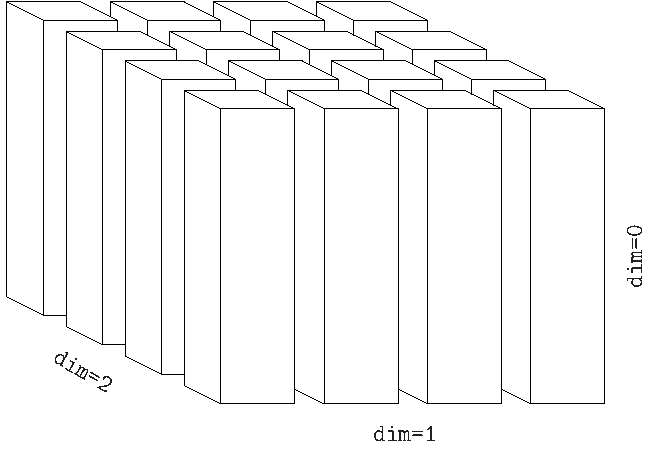
\includegraphics[width=0.42\textwidth]{latfield}
 \caption{\small Sketch of the domain decomposition performed by \textit{LATfield2} to distribute the work over the MPI processes. The data
 is stored in row-major order such that \texttt{dim=0} is \textit{contiguous} and \textit{local}, i.e.\ the non-contiguous dimensions
 \texttt{dim=1,2} are scattered over the process grid. This is essential for the FFT algorithm. In order to perform a 3D FFT,
 \textit{LATfield2} first computes a real-to-complex FFT for \texttt{dim=0}; then it performs a transposition between \texttt{dim=0} and
 \texttt{dim=1}, making the latter one the local dimension; then a complex-to-complex FFT is computed for the now-local \texttt{dim=1}; a
 second transposition between \texttt{dim=2} and \texttt{dim=1} makes \texttt{dim=2} finally local, and another complex-to-complex FFT is
 performed; in a last step, \textit{LATfield2} performs a transposition between the now-local \texttt{dim=2} and \texttt{dim=0} in order to
 make the latter one local again. Note that after these operations the 
ordering between \texttt{dim=1} and \texttt{dim=2} has been exchanged, but the \texttt{rKSite} class is aware of this. The number of \textit{k}-space points in the local \texttt{dim=0} is \texttt{Ngrid}/2 + 1. The backwards FFT carries out the operations in reverse order.}
\end{SCfigure}
 
 There are two ways to initialize a \texttt{Lattice}: either you specify the geometry, or you define a \texttt{Lattice} to be the Fourier
 image of an existing \texttt{Lattice} (the geometry follows automatically in this case). 
 
 \item[] \hspace{-25pt}\texttt{Site} ~ This class essentially represents a grid coordinate and provides a simple way to navigate the 3D
 data. There are two related classes, \texttt{rKSite} and \texttt{cKSite}, which are used to navigate the Fourier lattices of a real-to
 complex or complex-to-complex Fourier transform, respectively.
 
 \item[] \hspace{-25pt}\texttt{Field} ~ This class represents \textit{data} living on a \texttt{Lattice}. It could be a scalar field (real
 or complex) or a vector/tensor field. In \textit{gevolution} all fields live on the same \texttt{Lattice} (or its Fourier image).
 
 \textbf{Important}: any time a \texttt{Field} is modified locally and this modification should become ``effective'' globally, you have to
 call \texttt{updateHalo} for that \texttt{Field}. This will do the necessary communication between processes holding adjacent domains such
 that the halo sites have valid values.
 
 \item[] \hspace{-25pt}\texttt{PlanFFT} ~ This class is one of the centerpieces of \textit{LATfield2}. It connects a \texttt{Field} defined
 on a (configuration-space) \texttt{Lattice} with its Fourier image (living on the Fourier \texttt{Lattice}). A plan can be executed in
 either direction (\texttt{FFT\_FORWARD} / \texttt{FFT\_BACKWARD}), meaning that either the Fourier image or its counterpart will be
 computed by (inverse) FFT. The conventions for the FFT are exactly as in the \textit{FFTW} library (in particular, the FFT is unnormalized,
 meaning that a forward and backward transform together multiply a field by \texttt{Ngrid}$^\mathsf{3}$). Note that a FFT does not
 automatically update the \textit{halo}, so make sure to call \texttt{updateHalo} if appropriate.
 
 \item[] \hspace{-25pt}\texttt{Particles} ~ This class handles N-body particles in \textit{LATfield2}. The information about each particle
 is stored in a structure which contains the six phase-space coordinates (\texttt{pos[3]} and \texttt{vel[3]}, note that \texttt{vel[3]} is
 not a velocity vector in \textit{gevolution}, but rather a canonical momentum). These coordinates are updated by two functions,
 \texttt{updateVel} and \texttt{moveParticles}. Each of these functions loops over the particles and executes an update through a custom
 procedure passed as function pointer.
 
 Note that \textit{gevolution} uses the derived class \texttt{Particles\_gevolution} which additionally provides the I/O routine to write
 binary \textit{Gadget-2} format.
 
\end{itemize}

\noindent \textit{LATfield2} instantiates an object called \texttt{parallel} which can be used to manage communication between MPI
processes. This object is aware of the layout of the two-dimensional process grid used for the domain decomposition. Note that
\texttt{dim=2} of the \texttt{Lattice} is scattered along \texttt{dim=0} of the process grid!


\subsection{Navigating the source code}

The source code of \textit{gevolution} consists of several \textit{header} files and a \textit{main}. Subroutines and data structures are grouped in the header files according to purpose:

\begin{itemize}
 \item[] \hspace{-25pt}\texttt{background.hpp} ~ This header contains auxiliary functions related to the background model. In particular, it
 provides a fourth-order Runge-Kutta integrator for the scale factor. If the background model is modified, this should be done in this
 header.
 
 \item[] \hspace{-25pt}\texttt{class\_tools.hpp} ~ The interface with the Boltzmann code \textit{CLASS} is found in this header. It is only
 available if \textit{CLASS} is linked as a library and the compilation flag \texttt{-DHAVE\_CLASS} is specified.
 
 \item[] \hspace{-25pt}\texttt{gevolution.hpp} ~ This header contains the algorithms needed for the evolution of the metric and the solution
 of the geodesic equations for the N-body particles. If additional equations of motion for new degrees of freedom need to be implemented,
 one may add them here (or one creates a separate header).
 
 \item[] \hspace{-25pt}\texttt{hibernation.hpp} ~ This header contains the routines needed for writing a hibernation point to disk.
 
 \item[] \hspace{-25pt}\texttt{ic\_basic.hpp} ~ This header contains the \texttt{basic} IC generator and some auxiliary functions related to
 IC generation. Every IC generator, e.g.\ added by users for whatever purpose, should have a separate header file containing its source
 code.
 
 \item[] \hspace{-25pt}\texttt{ic\_prevolution.hpp} ~ This header contains the \texttt{prevolution} IC generator. It is only included when
 the compilation flag \texttt{-DICGEN\_PREVOLUTION} is specified.
 
 \item[] \hspace{-25pt}\texttt{ic\_read.hpp} ~ This header contains a function to read initial data from disk.
 
 \item[] \hspace{-25pt}\texttt{metadata.hpp} ~ This header defines some data structures which hold simulation parameters or settings related
 to IC generation. These data structures may have to be extended to include new parameters which arise when one implements additional
 physics. Most numerical constants are also defined in this header.
 
 \item[] \hspace{-25pt}\texttt{output.hpp} ~ This header contains the routines which produce output in form of snapshots or power spectra.
 
 \item[] \hspace{-25pt}\texttt{parser.hpp} ~ This header contains the parser for the settings file. The parser translates the information
 given in the settings file into the format used by the code and fills the data structures defined in \texttt{metadata.hpp} accordingly.
 Therefore, if new parameters are added, the parser needs to be modified in order to recognize them.
 
 \item[] \hspace{-25pt}\texttt{Particles\_gevolution.hpp} ~ This header defines the particle handler used by \textit{gevolution}. It is
 derived from the \texttt{Particles} class provided by \textit{LATfield2}, adding an I/O routine for \textit{Gadget-2} binary format.
 
 \item[] \hspace{-25pt}\texttt{radiation.hpp} ~ This header contains the linear radiation module. It is only enabled if the code is
 compiled with \texttt{-DHAVE\_CLASS}, linking \textit{CLASS} as a library.
 
 \item[] \hspace{-25pt}\texttt{tools.hpp} ~ This header contains auxiliary functions and tools, e.g.\ algorithms to compute power spectra and generate formatted output.
\end{itemize}

\paragraph{Main control sequence.} The main control sequence of \textit{gevolution} is found in \texttt{main.cpp}. It is structured as follows:

\begin{itemize}
 \item Initialization and parsing of settings file
 \item Generation of initial conditions ``on the fly'' %(lines \texttt{263}-\texttt{281})
 \item Main loop %(line \texttt{324})
% \begin{itemize}
%  \item Construction of stress-energy tensor of the N-body ensemble (lines \texttt{329}-\texttt{349})
%  \item Output of \textit{snapshots} (lines \texttt{357}-\texttt{593})
%  \item Output of \textit{power spectra} (lines \texttt{600}-\texttt{826})
%  \item Update $\mathsf{\Phi}$ (lines \texttt{853} and \texttt{864}, or line \texttt{877} for a \textit{Newtonian} run; the backwards FFT is done in line \texttt{883} for both cases, followed by \texttt{updateHalo} in line \texttt{888})
%  \item Output of \textit{background data} (lines \texttt{890}-\texttt{907})
%  \item Compute $\mathsf{\chi}$ (lines \texttt{911} and \texttt{922}; the backwards FFT is done in line \texttt{929}, followed by \texttt{updateHalo} in line \texttt{934})
%  \item Update B$_\mathsf{i}$ (line \texttt{924}; the backwards FFT is done in line \texttt{944} and \texttt{updateHalo} in line \texttt{949}) -- note that a copy of [\textit{a}$^\mathsf{2}$ B$_\mathsf{i}$] is kept in Fourier space in order for the solver to work (for all other fields, the Fourier image can usually be discarded after the backwards transform)
%  \item Update $\mathsf{\Psi}$ (lines \texttt{938}-\texttt{957})
%  \item Determine time step subdivision for non-CDM species (lines \texttt{959}-\texttt{975})
%  \item Update N-body particles (momenta and positions) using leap-frog (lines \texttt{997}-\texttt{1099}) -- the background is also evolved in this code section (lines \texttt{1063} and \texttt{1098})
%  \item $\mathsf{\tau}$ \texttt{+=} $\mathsf{\Delta\tau}$ and determine $\mathsf{\Delta\tau}$ for the next time step (lines \texttt{1111}-\texttt{1124})
% \end{itemize}
% \item The main loop terminates when no more output is scheduled (line \texttt{909})
 \item Cleanup
\end{itemize}

\noindent The general procedure for adding new physics is the following. First, one needs to implement a way to handle the additional
degrees of freedom -- in many cases the \texttt{Field} class can be useful for this purpose. Then one needs a procedure to construct the
stress-energy tensor for the configuration of the additional degrees of freedom. This new contribution to the stress-energy tensor needs to
be added at an appropriate point in the main loop. The code will then proceed to evolve the metric according to the new stress-energy
sources. Finally, one needs to implement an algorithm to solve the equations of motion for the new degrees of freedom. This will generally
depend on the metric and should therefore be called after the metric is evolved, probably somewhere close to the particle update.

In addition, one will also have to write a new IC generator which includes the new degrees of freedom, and possibly some new output routines
if additional quantities are to be studied.

\subsection{Code units}
\label{sec:units}

The code works in natural units where \textit{c} = 1. Both, conformal distances and conformal time are measured in units of the comoving box
size (i.e.\ spatial coordinates range between 0 and 1). Metric perturbations are dimensionless. The canonical momentum is measured in units
of the particle mass in order to make it dimensionless and independent of the mass resolution.

For the stress-energy tensor the code actually computes -\textit{a}$^\mathsf{3} \mathsf{T^0_0}$ and \textit{a}$^\mathsf{3} \mathsf{T^i_j}$,
i.e.\ the background expansion is scaled out. Also, the mass units are chosen such that, in the homogeneous limit and for nonrelativistic
matter, the -\textit{a}$^\mathsf{3}\mathsf{\bar{T}^0_0}$ is equal its density parameter $\mathsf{\Omega}$ at redshift \textit{z} = 0.

When output power spectra are computed, the code always writes the dimensionless spectra as defined in \cite{Adamek:2015eda}. However,
\textit{k} is converted back to physical units, \textit{h}/Mpc. Particle snapshots in \textit{Gadget-2} format use length units of
kpc/\textit{h}, mass units of 10$^\mathsf{10}$ \textit{M}$_\odot$/\textit{h} and velocities in km/s. These can be adjusted with the compiler
flags \texttt{-DGADGET\_LENGTH\_CONVERSION=}\textit{<value>}, \texttt{-DGADGET\_MASS\_CONVERSION=}\textit{<value>} and
\texttt{-DGADGET\_VELOCITY\_CONVERSION=}\textit{<value>}. HDF5 output is produced in code units.

\section{Patches}

Minor bugs will be addressed with patches on the \textit{master} branch of the repository. Apart from that, the features of each version of
the code should remain stable. New features are implemented on a separate branch which may eventually become a new release version of the
code.

%\paragraph{Patch 1} (April 2016)
%\begin{itemize}
% \item Fixed minor bugs in \texttt{parser.hpp} and \texttt{ic\_basic.hpp} which affected simulations with more than one particle species.
% \item Changed default batch size for writing particles in \textit{Gadget-2} format from \texttt{1024} to \texttt{1048576}. This is an
% optimization parameter which can be manually set by adding \texttt{-DPCLBUFFER=}\textit{<value>} as compiler option.
% \item The particle number in \textit{Gadget-2} format is now interpreted as unsigned integer, allowing for files with up to 4 billion
% particles (the previous maximum file size was about 2 billion particles).
% \item Added \texttt{-std=c++11} as compiler flag in the \texttt{makefile}. This is required by the current version of the \textit{LATfield2}
% library.
%\end{itemize}


\bibliographystyle{utcaps}
\bibliography{manual}

\end{document}
